\chapter{Comment mettre en place une connection paire à paire}

\section{Avec WebRTC}

\paragraph{}
L'utilisation de WebRTC est l'une des solutions possibles pour mettre en place une communication textuelle en temps réel entre deux clients dans un réseau pair à pair.
Pour établir cette connexion, les étapes suivantes peuvent être suivies :

\subsection{Initialisation d'une paire et récupération de son ID}

\paragraph{}
Chaque client doit être initialisé en tant que paire et se voit attribuer un ID unique. Cet ID est utilisé pour identifier la paire et permettre à d'autres pairs de se connecter à elle.

\subsection{Partage des ID entre les deux pairs}

\paragraph{}
Une fois que chaque paire a obtenu son ID, ces identifiants doivent être partagés entre les deux pairs afin qu'ils puissent s'identifier mutuellement lors de l'établissement de la connexion. 
Cela peut être réalisé par l'intermédiaire d'un serveur de signalisation ou d'un canal de communication préalablement établi, tel qu'un serveur centralisé ou un autre moyen de communication sécurisé.

\subsection{Création d'une connexion entre les deux pairs}

\paragraph{}
Une fois que chaque pair dispose de l'ID de l'autre, ils peuvent utiliser ce dernier pour établir une connexion directe entre eux. 

\subsection{Echange de données entre les deux pairs}

\paragraph{}
Une fois la connexion établie, les deux pairs peuvent s'échanger des données. Ces données peuvent être des messages textuels, des fichiers, des flux audio et vidéo, etc. 
(Dans notre cas, nous nous intéressons uniquement aux messages textuels.)


\begin{figure}[h]
    \centering
    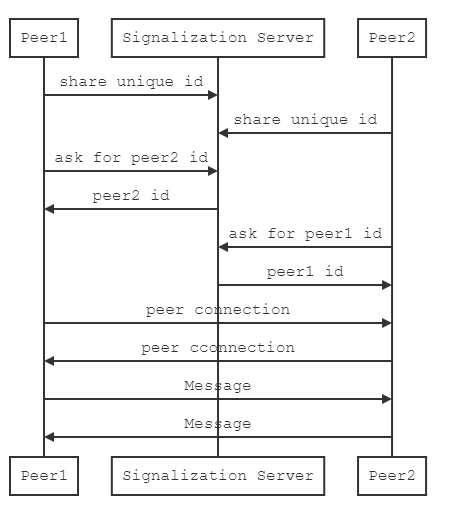
\includegraphics[width=0.8\textwidth]{assets/webrtc_connection.png}
    \caption{Schéma de fonctionnement de WebRTC}
    \label{fig:webrtc}
\end{figure}

\newpage 

\section{Avec WebSockets}

\paragraph{}
Une autre solution pour mettre en place une communication textuelle en temps réel entre deux clients dans un réseau pair à pair est d'utiliser les WebSockets.
La principale difference avec WebRTC, c'est que les Sockets nécessitent la connaissance des adresses IP des deux pairs pour pouvoir établir une connexion entre eux.
Pour établir cette connexion, les étapes suivantes peuvent être suivies :

\subsection{Récupération de l'adresse IP publique du client}

\paragraph{}
Pour pouvoir établir une connexion entre deux pairs, il faut que chaque pair connaisse l'adresse IP publique ainsi que le port utilisé par l'autre pair. Mais avant cela, il faut que chaque pair récupère son adresse IP publique afin
de la partager avec l'autre pair. Pour cela, il existe une solution (non unique) qui consiste à utiliser un service STUN qui permet de récupérer l'adresse IP publique du client ainsi qu'un port ouvert sur le pare-feu du client.

\subsection{Partage des adresses IP entre les deux pairs}

\paragraph{}
Une fois ces informations récupérées, chaque pair doit partager son adresse IP publique ainsi que le port ouvert sur son pare-feu avec l'autre pair. Cela peut être réalisé par l'intermédiaire d'un serveur de signalisation 
ou d'un canal de communication préalablement établi, tel qu'un serveur centralisé ou un autre moyen de communication sécurisé.

\subsection{Création d'une connexion entre les deux pairs}

\paragraph{}
Une fois que chaque pair dispose de l'adresse IP publique et du port ouvert sur le pare-feu de l'autre pair, ils peuvent utiliser ces informations pour établir une connexion directe entre eux. 

\subsection{Echange de données entre les deux pairs}

\paragraph{}
Une fois la connexion établie, les deux pairs peuvent s'échanger des données. Ces données peuvent être des messages textuels, des fichiers, des flux audio et vidéo, etc.
(Dans notre cas, nous nous intéressons uniquement aux messages textuels.)

\begin{figure}[h]
    \centering
    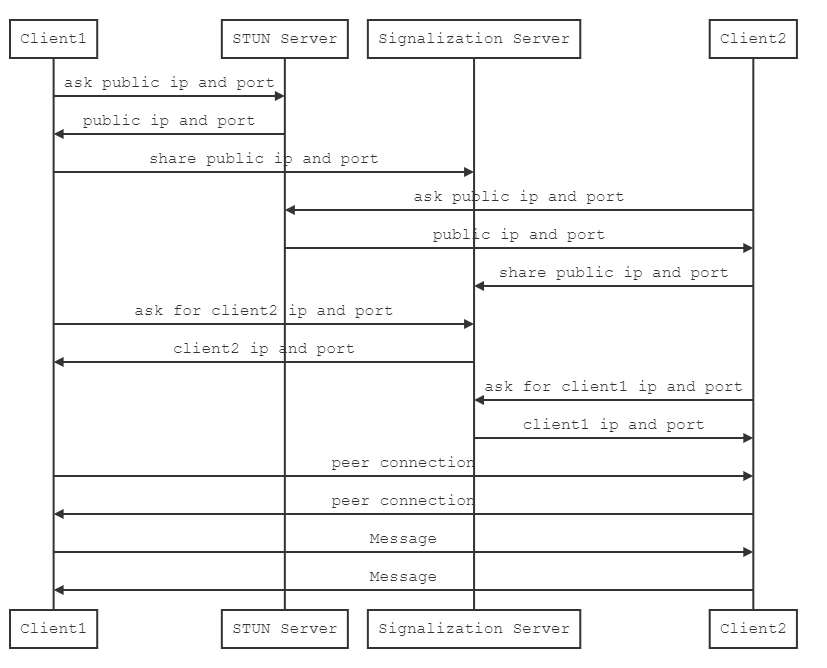
\includegraphics[width=0.99\textwidth]{assets/socket_connection.png}
    \caption{Schéma de fonctionnement de WebSockets}
    \label{fig:websockets}
\end{figure}


\section{Les outils tiers nécessaires pour la communication pair à pair}

\subsection{Les serveurs de signalisation}

\paragraph{}
Pour établir une communication pair à pair entre deux clients, il est souvent nécessaire de mettre en place des serveurs de signalisation. Les serveurs de signalisation agissent comme des intermédiaires pour faciliter 
l'établissement de la connexion initiale entre les clients.

\paragraph{}
Lorsqu'un client souhaite établir une communication avec un autre client, il doit d'abord échanger des informations telles que les adresses IP et les ports. Les serveurs de signalisation permettent aux clients de partager ces 
informations entre eux. Ils peuvent également aider à coordonner les étapes de négociation et d'établissement de la connexion.

\paragraph{}
Les serveurs de signalisation peuvent utiliser différents protocoles et techniques pour échanger les informations nécessaires. Par exemple, ils peuvent utiliser des protocoles basés sur le web tels que HTTP pour envoyer des messages 
de signalisation entre les clients. Ils peuvent également utiliser des protocoles de signalisation spécialisés tels que SIP (Session Initiation Protocol) ou XMPP (Extensible Messaging and Presence Protocol).

\paragraph{}
Il existe différentes options pour mettre en place des serveurs de signalisation, allant des solutions prêtes à l'emploi aux serveurs personnalisés développés en interne. Certains services cloud offrent également des 
fonctionnalités de signalisation pour faciliter l'établissement de connexions pair à pair.

\paragraph{}
Il est important de noter que les serveurs de signalisation ne sont généralement pas impliqués dans le transfert direct des données entre les clients. Ils jouent simplement un rôle de coordination pour permettre 
l'établissement de la connexion initiale.


\subsection{Les protocoles TURN et STUN}

Pour faciliter les communications pair à pair, il est souvent nécessaire de prendre en compte les contraintes de réseau telles que les pare-feu et les NAT (Network Address Translation). Deux protocoles couramment utilisés pour résoudre ces 
problèmes sont TURN (Traversal Using Relays around NAT) et STUN (Session Traversal Utilities for NAT).

\paragraph{}
Le protocole STUN permet à un client d'obtenir des informations sur son adresse IP publique et le type de NAT qu'il traverse. Cela permet au client de comprendre comment il est connecté au réseau et d'adapter ses stratégies de 
connexion en conséquence. STUN est généralement utilisé pour faciliter l'établissement de connexions pair à pair lorsque les clients sont derrière des NAT symétriques ou des pare-feu restrictifs.

\paragraph{}
Le protocole TURN est utilisé lorsque les connexions pair à pair directes ne sont pas possibles en raison de pare-feu ou de NAT restrictifs. TURN utilise un serveur intermédiaire (relais) auquel les clients se connectent pour acheminer 
leurs données. Ce serveur intermédiaire agit comme un proxy et transfère les données entre les clients. Cela permet aux clients de communiquer même s'ils ne peuvent pas établir une connexion directe.

\paragraph{}
Lorsqu'un client rencontre des difficultés pour établir une connexion pair à pair directe en raison des restrictions du réseau, il peut utiliser STUN pour obtenir son adresse IP publique, puis essayer d'établir une connexion directe. 
Si cela échoue, le client peut passer à l'utilisation de TURN pour acheminer les données via un serveur relais.

\paragraph{}
Il est important de noter que l'utilisation de TURN peut entraîner une latence supplémentaire car les données doivent être acheminées via le serveur relais. De plus, l'utilisation d'un serveur relais peut entraîner des coûts supplémentaires, 
notamment si vous utilisez un service cloud ou un fournisseur tiers pour héberger le serveur.

\paragraph{}
En résumé, les protocoles TURN et STUN sont des outils importants pour faciliter les communications pair à pair lorsque les clients sont derrière des NAT restrictifs ou des pare-feu. Ils permettent de contourner les contraintes réseau et de 
faciliter l'établissement de connexions directes ou le transfert des données via un serveur relais lorsque cela est nécessaire.


\subsection{Les serveurs de relais}

\paragraph{}
Dans certains cas, il peut être nécessaire d'utiliser des serveurs de relais pour faciliter la communication pair à pair. Les serveurs de relais agissent comme des intermédiaires pour acheminer les données entre les 
clients lorsque des connexions directes ne sont pas possibles en raison de restrictions de pare-feu, de problèmes de NAT (Network Address Translation) ou d'autres contraintes réseau.

\paragraph{}
Lorsqu'un client ne peut pas établir une connexion directe avec un autre client en raison de ces contraintes, il peut utiliser un serveur de relais pour envoyer ses données vers le serveur, qui les transférera ensuite au client destinataire.

\paragraph{}
Les serveurs de relais peuvent être mis en place de différentes manières. Certains services cloud proposent des serveurs de relais prêts à l'emploi, tandis que d'autres solutions nécessitent la configuration de serveurs dédiés pour le relais des données.

\paragraph{}
L'utilisation de serveurs de relais peut être bénéfique dans certains scénarios où les connexions directes entre les clients ne sont pas possibles. Cependant, cela introduit généralement une surcharge supplémentaire et peut augmenter la latence de la communication.

\paragraph{}
En étudiant ces outils tiers nécessaires pour la communication pair à pair, nous pourrons mieux comprendre comment ils peuvent être intégrés dans notre solution de communication textuelle temps réel. Cela nous permettra d'explorer les fonctionnalités, 
les avantages et les limites de chaque outil, et d'évaluer leur pertinence pour notre projet.


